\subsection{Scenario 2: Risk Introduction}
\textit{This scenario introduces a risk to the infrastructure after $180$ seconds. The purpose of this scenario is to see how the system behaves when a new risk is introduced.}

\begin{figure}[H]
    \centering
    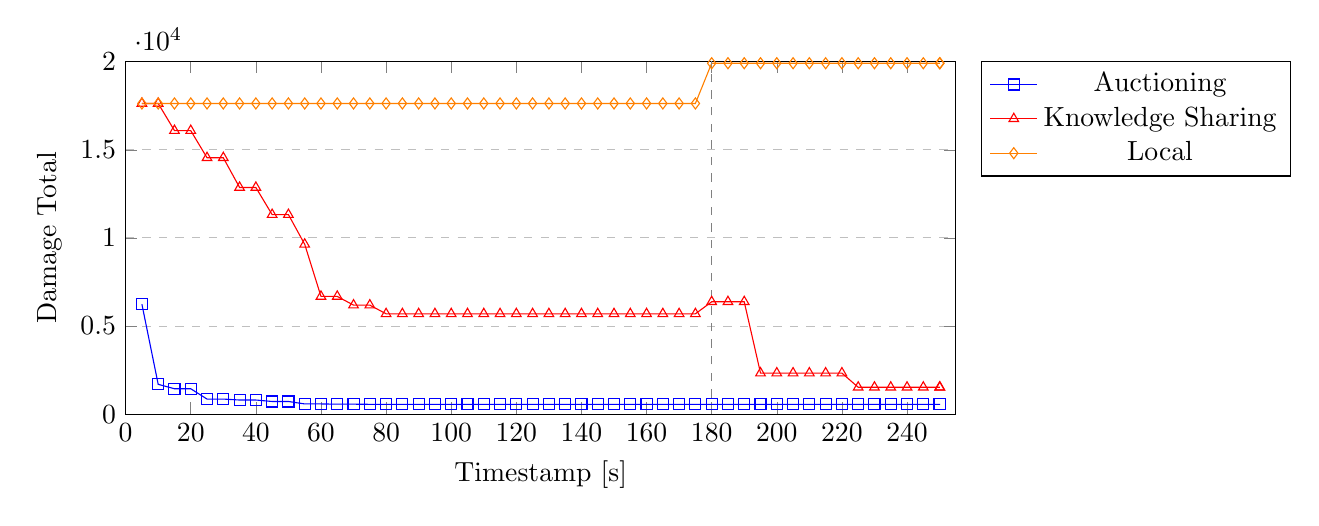
\begin{tikzpicture}
\begin{axis}[
    xlabel={Timestamp [s]},
    ylabel={Damage Total},
    xmin=0, xmax=255000,
    ymin=0, ymax=20020,
    legend pos=outer north east,
    ymajorgrids=true,
    grid style=dashed,
    width=\textwidth,
    height=0.5\textwidth,
    scaled x ticks=base 10:-3,
    xtick scale label code/.code={}
]

	\addplot[color=blue,mark=square] coordinates {
        (5000,6236.51)(10000,1693.70)(15000,1442.78)(20000,1442.78)(25000,857.00)(30000,857.00)(35000,803.10)(40000,803.10)(45000,720.33)(50000,720.33)(55000,580.88)(60000,580.88)(65000,567.64)(70000,567.64)(75000,559.15)(80000,556.95)(85000,556.95)(90000,556.95)(95000,556.95)(100000,556.95)(105000,556.95)(110000,556.95)(115000,556.95)(120000,556.95)(125000,556.95)(130000,556.95)(135000,556.95)(140000,556.95)(145000,556.95)(150000,556.95)(155000,556.95)(160000,556.95)(165000,556.95)(170000,556.95)(175000,556.95)(180000,556.95)(185000,560.22)(190000,560.22)(195000,560.22)(200000,560.22)(205000,560.22)(210000,560.22)(215000,560.22)(220000,560.22)(225000,560.22)(230000,560.22)(235000,560.22)(240000,560.22)(245000,560.22)(250000,560.22)(250139,560.22)
    };
    \addlegendentry{Auctioning}
	\addplot[color=red,mark=triangle] coordinates {
        (5000,17629.95)(10000,17629.95)(15000,16089.24)(20000,16089.24)(25000,14548.54)(30000,14548.54)(35000,12864.04)(40000,12864.04)(45000,11323.33)(50000,11323.33)(55000,9638.83)(60000,6680.68)(65000,6680.68)(70000,6187.65)(75000,6187.65)(80000,5694.63)(85000,5694.63)(90000,5694.63)(95000,5694.63)(100000,5694.63)(105000,5694.63)(110000,5694.63)(115000,5694.63)(120000,5694.63)(125000,5694.63)(130000,5694.63)(135000,5694.63)(140000,5694.63)(145000,5694.63)(150000,5694.63)(155000,5694.63)(160000,5694.63)(165000,5694.63)(170000,5694.63)(175000,5694.63)(180000,6377.52)(185000,6377.52)(190000,6377.52)(195000,2331.23)(200000,2331.23)(205000,2331.23)(210000,2331.23)(215000,2331.23)(220000,2331.23)(225000,1526.78)(230000,1526.78)(235000,1526.78)(240000,1526.78)(245000,1526.78)(250000,1526.78)(250111,1526.78)
    };
    \addlegendentry{Knowledge Sharing}
	\addplot[color=orange,mark=diamond] coordinates {
        (5000,17629.95)(10000,17629.95)(15000,17629.95)(20000,17629.95)(25000,17629.95)(30000,17629.95)(35000,17629.95)(40000,17629.95)(45000,17629.95)(50000,17629.95)(55000,17629.95)(60000,17629.95)(65000,17629.95)(70000,17629.95)(75000,17629.95)(80000,17629.95)(85000,17629.95)(90000,17629.95)(95000,17629.95)(100000,17629.95)(105000,17629.95)(110000,17629.95)(115000,17629.95)(120000,17629.95)(125000,17629.95)(130000,17629.95)(135000,17629.95)(140000,17629.95)(145000,17629.95)(150000,17629.95)(155000,17629.95)(160000,17629.95)(165000,17629.95)(170000,17629.95)(175000,17629.95)(180000,19913.02)(185000,19913.02)(190000,19913.02)(195000,19913.02)(200000,19913.02)(205000,19913.02)(210000,19913.02)(215000,19913.02)(220000,19913.02)(225000,19913.02)(230000,19913.02)(235000,19913.02)(240000,19913.02)(245000,19913.02)(250000,19913.02)(250115,19913.02)
    };
    \addlegendentry{Local}

	\addplot[color=gray, dashed,] coordinates {(180000,0) (180000,20020)};


\end{axis}
\end{tikzpicture}
    \caption{This graph shows the overall damage of the system in the risk introduction scenario. The damage is shown for each of the three strategies. The vertical lines indicate the time at which a risk is introduced.}
    \label{fig:overall-damage-inroduce-risk}
\end{figure}

Figure \ref{fig:overall-damage-inroduce-risk} shows a graph that follows a similar trend as shown in figure \ref{fig:overall-damage-no-change}. This is to be expected as the scenarios are identical up until the $180$ seconds mark. During this time we see a small increase in damage for all graphs. As the metrics are collected in $5000$ms intervals, it is not obvious from the graph that an increase in damage occurs. However, when observing the logs of each agent the damage increase can be seen. 

\begin{figure}[H]
    \centering
    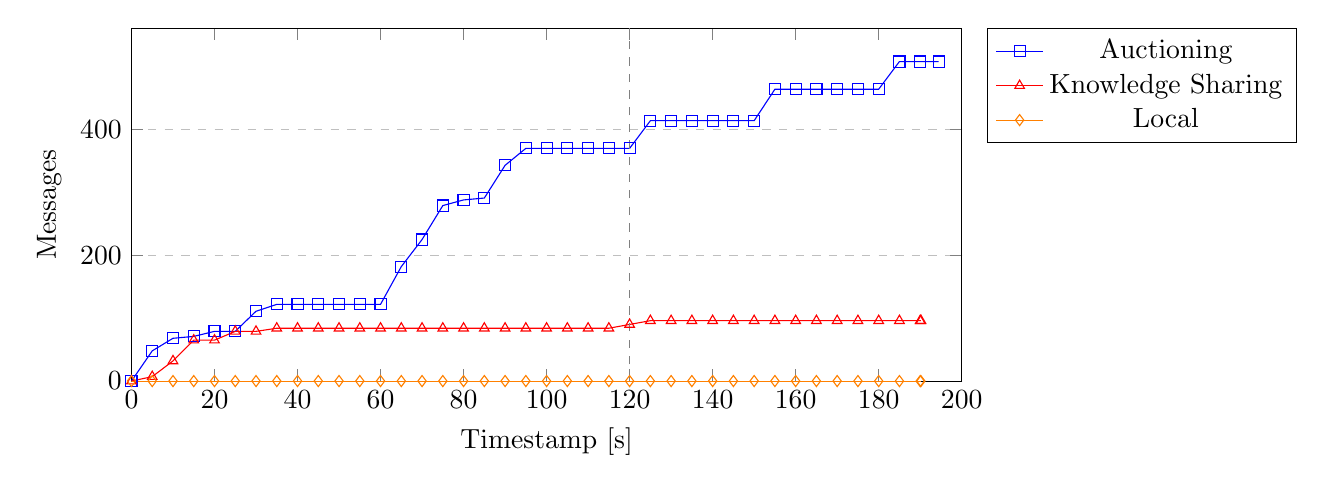
\begin{tikzpicture}
\begin{axis}[
    xlabel={Timestamp [s]},
    ylabel={Messages},
    xmin=0, xmax=200000,
    ymin=0, ymax=561,
    legend pos=outer north east,
    ymajorgrids=true,
    grid style=dashed,
    width=\textwidth,
    height=0.5\textwidth,
    scaled x ticks=base 10:-3,
    xtick scale label code/.code={}
]

	\addplot[color=blue,mark=square] coordinates {
        (0,0)(5000,48)(10000,68)(15000,71)(20000,79)(25000,79)(30000,111)(35000,122)(40000,122)(45000,122)(50000,122)(55000,122)(60000,122)(65000,182)(70000,225)(75000,279)(80000,288)(85000,291)(90000,343)(95000,370)(100000,370)(105000,370)(110000,370)(115000,370)(120000,370)(125000,414)(130000,414)(135000,414)(140000,414)(145000,414)(150000,414)(155000,464)(160000,464)(165000,464)(170000,464)(175000,464)(180000,464)(185000,508)(190000,508)(194440,508)
    };
    \addlegendentry{Auctioning}
	\addplot[color=red,mark=triangle] coordinates {
        (0,0)(5000,7)(10000,32)(15000,65)(20000,65)(25000,79)(30000,79)(35000,84)(40000,84)(45000,84)(50000,84)(55000,84)(60000,84)(65000,84)(70000,84)(75000,84)(80000,84)(85000,84)(90000,84)(95000,84)(100000,84)(105000,84)(110000,84)(115000,84)(120000,90)(125000,96)(130000,96)(135000,96)(140000,96)(145000,96)(150000,96)(155000,96)(160000,96)(165000,96)(170000,96)(175000,96)(180000,96)(185000,96)(190000,96)(190192,96)
    };
    \addlegendentry{Knowledge Sharing}
	\addplot[color=orange,mark=diamond] coordinates {
        (0,0)(5000,0)(10000,0)(15000,0)(20000,0)(25000,0)(30000,0)(35000,0)(40000,0)(45000,0)(50000,0)(55000,0)(60000,0)(65000,0)(70000,0)(75000,0)(80000,0)(85000,0)(90000,0)(95000,0)(100000,0)(105000,0)(110000,0)(115000,0)(120000,0)(125000,0)(130000,0)(135000,0)(140000,0)(145000,0)(150000,0)(155000,0)(160000,0)(165000,0)(170000,0)(175000,0)(180000,0)(185000,0)(190000,0)(190162,0)
    };
    \addlegendentry{Local}

	\addplot[color=gray, dashed,] coordinates {(120000,0) (120000,561)};


\end{axis}
\end{tikzpicture}
    \caption{Graph showing the total amount of messages sent between agents in the risk introduction scenario.}
    \label{fig:messages-risk-introduction}
\end{figure}
\begin{figure}[H]
    \centering
    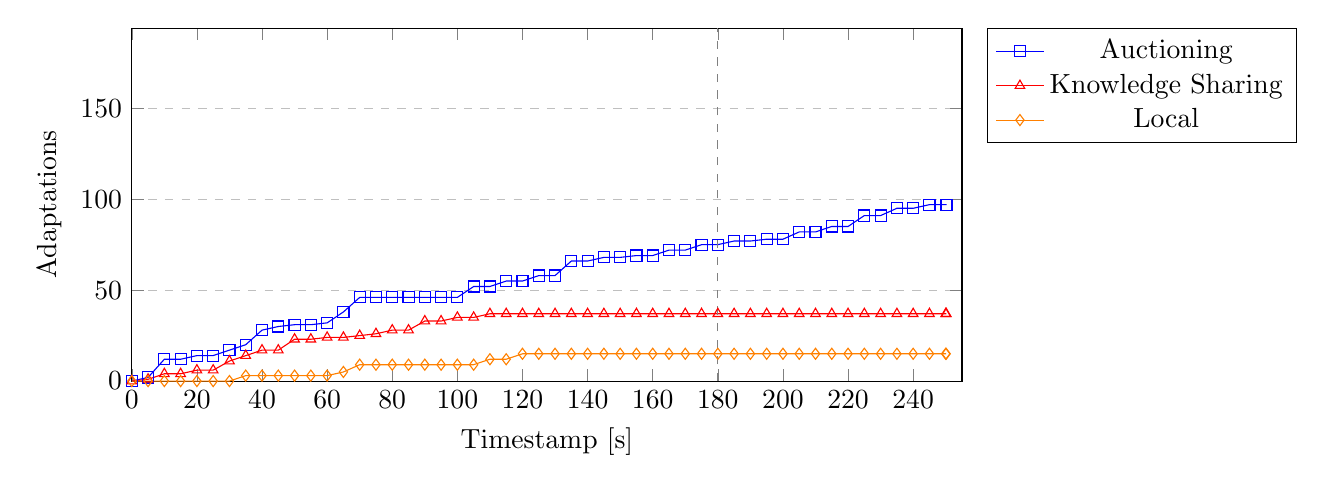
\begin{tikzpicture}
\begin{axis}[
    xlabel={Timestamp [s]},
    ylabel={Adaptations},
    xmin=0, xmax=255000,
    ymin=0, ymax=194,
    legend pos=outer north east,
    ymajorgrids=true,
    grid style=dashed,
    width=\textwidth,
    height=0.5\textwidth,
    scaled x ticks=base 10:-3,
    xtick scale label code/.code={}
]

	\addplot[color=blue,mark=square] coordinates {
        (0,0)(5000,2)(10000,12)(15000,12)(20000,14)(25000,14)(30000,17)(35000,20)(40000,28)(45000,30)(50000,31)(55000,31)(60000,32)(65000,38)(70000,46)(75000,46)(80000,46)(85000,46)(90000,46)(95000,46)(100000,46)(105000,52)(110000,52)(115000,55)(120000,55)(125000,58)(130000,58)(135000,66)(140000,66)(145000,68)(150000,68)(155000,69)(160000,69)(165000,72)(170000,72)(175000,75)(180000,75)(185000,77)(190000,77)(195000,78)(200000,78)(205000,82)(210000,82)(215000,85)(220000,85)(225000,91)(230000,91)(235000,95)(240000,95)(245000,97)(250000,97)(250288,97)
    };
    \addlegendentry{Auctioning}
	\addplot[color=red,mark=triangle] coordinates {
        (0,0)(5000,1)(10000,4)(15000,4)(20000,6)(25000,6)(30000,11)(35000,14)(40000,17)(45000,17)(50000,23)(55000,23)(60000,24)(65000,24)(70000,25)(75000,26)(80000,28)(85000,28)(90000,33)(95000,33)(100000,35)(105000,35)(110000,37)(115000,37)(120000,37)(125000,37)(130000,37)(135000,37)(140000,37)(145000,37)(150000,37)(155000,37)(160000,37)(165000,37)(170000,37)(175000,37)(180000,37)(185000,37)(190000,37)(195000,37)(200000,37)(205000,37)(210000,37)(215000,37)(220000,37)(225000,37)(230000,37)(235000,37)(240000,37)(245000,37)(250000,37)(250159,37)
    };
    \addlegendentry{Knowledge Sharing}
	\addplot[color=orange,mark=diamond] coordinates {
        (0,0)(5000,0)(10000,0)(15000,0)(20000,0)(25000,0)(30000,0)(35000,3)(40000,3)(45000,3)(50000,3)(55000,3)(60000,3)(65000,5)(70000,9)(75000,9)(80000,9)(85000,9)(90000,9)(95000,9)(100000,9)(105000,9)(110000,12)(115000,12)(120000,15)(125000,15)(130000,15)(135000,15)(140000,15)(145000,15)(150000,15)(155000,15)(160000,15)(165000,15)(170000,15)(175000,15)(180000,15)(185000,15)(190000,15)(195000,15)(200000,15)(205000,15)(210000,15)(215000,15)(220000,15)(225000,15)(230000,15)(235000,15)(240000,15)(245000,15)(250000,15)(250135,15)
    };
    \addlegendentry{Local}

	\addplot[color=gray, dashed,] coordinates {(180000,0) (180000,194)};


\end{axis}
\end{tikzpicture}
    \caption{Graph showing the total amount of adaptations applied by agents in the risk introduction scenario.}
    \label{fig:proposals-risk-introduction}
\end{figure}

When the risk is introduced after $180$ seconds, we can see in Figure \ref{fig:proposals-risk-introduction} that no new adaptations are applied. We would expect at least a few adaptations to be made for the knowledge-sharing and auctioning agent. However, this is not the case.

\begin{figure}[H]
    \centering
        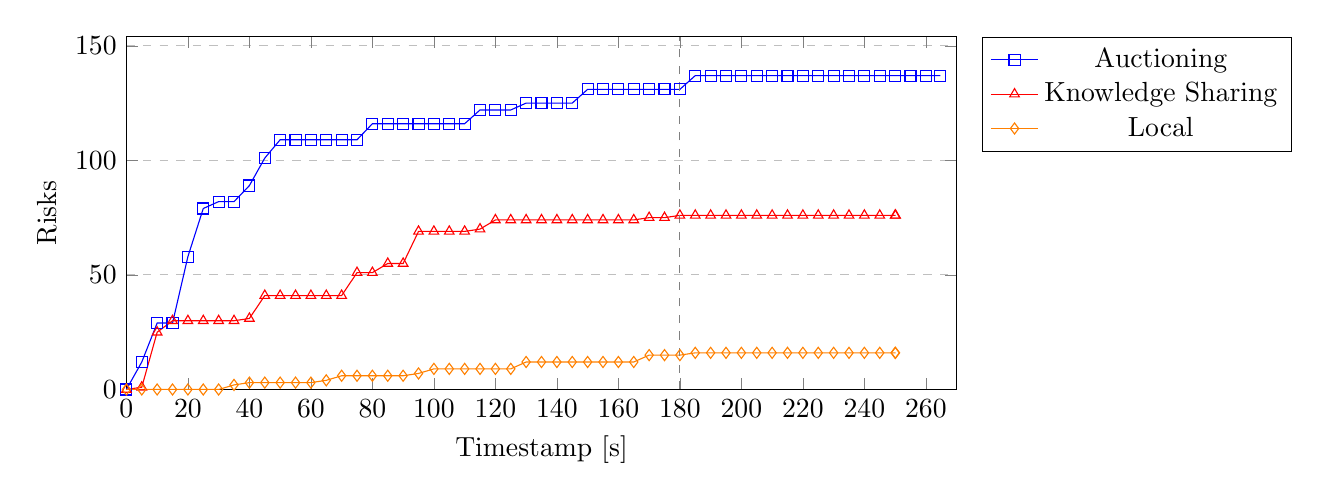
\begin{tikzpicture}
\begin{axis}[
    xlabel={Timestamp [s]},
    ylabel={Risks},
    xmin=0, xmax=270000,
    ymin=0, ymax=154,
    legend pos=outer north east,
    ymajorgrids=true,
    grid style=dashed,
    width=\textwidth,
    height=0.5\textwidth,
    scaled x ticks=base 10:-3,
    xtick scale label code/.code={}
]

	\addplot[color=blue,mark=square] coordinates {
        (0,0)(5000,12)(10000,29)(15000,29)(20000,58)(25000,79)(30000,82)(35000,82)(40000,89)(45000,101)(50000,109)(55000,109)(60000,109)(65000,109)(70000,109)(75000,109)(80000,116)(85000,116)(90000,116)(95000,116)(100000,116)(105000,116)(110000,116)(115000,122)(120000,122)(125000,122)(130000,125)(135000,125)(140000,125)(145000,125)(150000,131)(155000,131)(160000,131)(165000,131)(170000,131)(175000,131)(180000,131)(185000,137)(190000,137)(195000,137)(200000,137)(205000,137)(210000,137)(215000,137)(220000,137)(225000,137)(230000,137)(235000,137)(240000,137)(245000,137)(250000,137)(255000,137)(260000,137)(264723,137)
    };
    \addlegendentry{Auctioning}
	\addplot[color=red,mark=triangle] coordinates {
        (0,0)(5000,1)(10000,25)(15000,30)(20000,30)(25000,30)(30000,30)(35000,30)(40000,31)(45000,41)(50000,41)(55000,41)(60000,41)(65000,41)(70000,41)(75000,51)(80000,51)(85000,55)(90000,55)(95000,69)(100000,69)(105000,69)(110000,69)(115000,70)(120000,74)(125000,74)(130000,74)(135000,74)(140000,74)(145000,74)(150000,74)(155000,74)(160000,74)(165000,74)(170000,75)(175000,75)(180000,76)(185000,76)(190000,76)(195000,76)(200000,76)(205000,76)(210000,76)(215000,76)(220000,76)(225000,76)(230000,76)(235000,76)(240000,76)(245000,76)(250000,76)(250156,76)
    };
    \addlegendentry{Knowledge Sharing}
	\addplot[color=orange,mark=diamond] coordinates {
        (0,0)(5000,0)(10000,0)(15000,0)(20000,0)(25000,0)(30000,0)(35000,2)(40000,3)(45000,3)(50000,3)(55000,3)(60000,3)(65000,4)(70000,6)(75000,6)(80000,6)(85000,6)(90000,6)(95000,7)(100000,9)(105000,9)(110000,9)(115000,9)(120000,9)(125000,9)(130000,12)(135000,12)(140000,12)(145000,12)(150000,12)(155000,12)(160000,12)(165000,12)(170000,15)(175000,15)(180000,15)(185000,16)(190000,16)(195000,16)(200000,16)(205000,16)(210000,16)(215000,16)(220000,16)(225000,16)(230000,16)(235000,16)(240000,16)(245000,16)(250000,16)(250126,16)
    };
    \addlegendentry{Local}

	\addplot[color=gray, dashed,] coordinates {(180000,0) (180000,154)};


\end{axis}
\end{tikzpicture}
    \caption{Graph showing the number of unique risks detected by agents in the risk introduction scenario.}
    \label{fig:risk-count-risk-introduction}
\end{figure}
\begin{figure}[H]
    \centering
        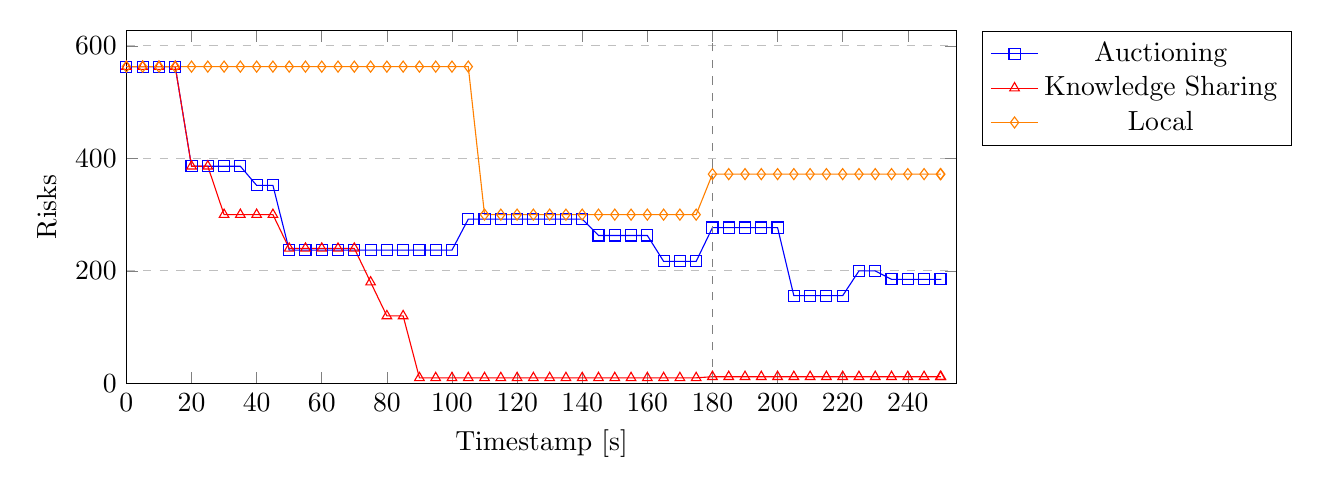
\begin{tikzpicture}
\begin{axis}[
    xlabel={Timestamp [s]},
    ylabel={Risks},
    xmin=0, xmax=255000,
    ymin=0, ymax=627,
    legend pos=outer north east,
    ymajorgrids=true,
    grid style=dashed,
    width=\textwidth,
    height=0.5\textwidth,
    scaled x ticks=base 10:-3,
    xtick scale label code/.code={}
]

	\addplot[color=blue,mark=square] coordinates {
        (0,563)(5000,563)(10000,563)(15000,563)(20000,386)(25000,386)(30000,386)(35000,386)(40000,352)(45000,352)(50000,237)(55000,237)(60000,237)(65000,237)(70000,237)(75000,237)(80000,237)(85000,237)(90000,237)(95000,237)(100000,237)(105000,292)(110000,292)(115000,292)(120000,292)(125000,292)(130000,292)(135000,292)(140000,292)(145000,263)(150000,263)(155000,263)(160000,263)(165000,217)(170000,217)(175000,217)(180000,277)(185000,277)(190000,277)(195000,277)(200000,277)(205000,156)(210000,156)(215000,156)(220000,156)(225000,200)(230000,200)(235000,185)(240000,185)(245000,185)(250000,185)(250288,185)
    };
    \addlegendentry{Auctioning}
	\addplot[color=red,mark=triangle] coordinates {
        (0,563)(5000,563)(10000,563)(15000,563)(20000,386)(25000,386)(30000,300)(35000,300)(40000,300)(45000,300)(50000,240)(55000,240)(60000,240)(65000,240)(70000,240)(75000,180)(80000,120)(85000,120)(90000,10)(95000,10)(100000,10)(105000,10)(110000,10)(115000,10)(120000,10)(125000,10)(130000,10)(135000,10)(140000,10)(145000,10)(150000,10)(155000,10)(160000,10)(165000,10)(170000,10)(175000,10)(180000,12)(185000,12)(190000,12)(195000,12)(200000,12)(205000,12)(210000,12)(215000,12)(220000,12)(225000,12)(230000,12)(235000,12)(240000,12)(245000,12)(250000,12)(250159,12)
    };
    \addlegendentry{Knowledge Sharing}
	\addplot[color=orange,mark=diamond] coordinates {
        (0,563)(5000,563)(10000,563)(15000,563)(20000,563)(25000,563)(30000,563)(35000,563)(40000,563)(45000,563)(50000,563)(55000,563)(60000,563)(65000,563)(70000,563)(75000,563)(80000,563)(85000,563)(90000,563)(95000,563)(100000,563)(105000,563)(110000,300)(115000,300)(120000,300)(125000,300)(130000,300)(135000,300)(140000,300)(145000,300)(150000,300)(155000,300)(160000,300)(165000,300)(170000,300)(175000,300)(180000,372)(185000,372)(190000,372)(195000,372)(200000,372)(205000,372)(210000,372)(215000,372)(220000,372)(225000,372)(230000,372)(235000,372)(240000,372)(245000,372)(250000,372)(250135,372)
    };
    \addlegendentry{Local}

	\addplot[color=gray, dashed,] coordinates {(180000,0) (180000,627)};


\end{axis}
\end{tikzpicture}
    \caption{Graph showing the number of remaining risks in the infrastructure in the risk introduction scenario.}
    \label{fig:risk-remaining-risk-introduction}
\end{figure}
\begin{figure}[H]
    \centering
        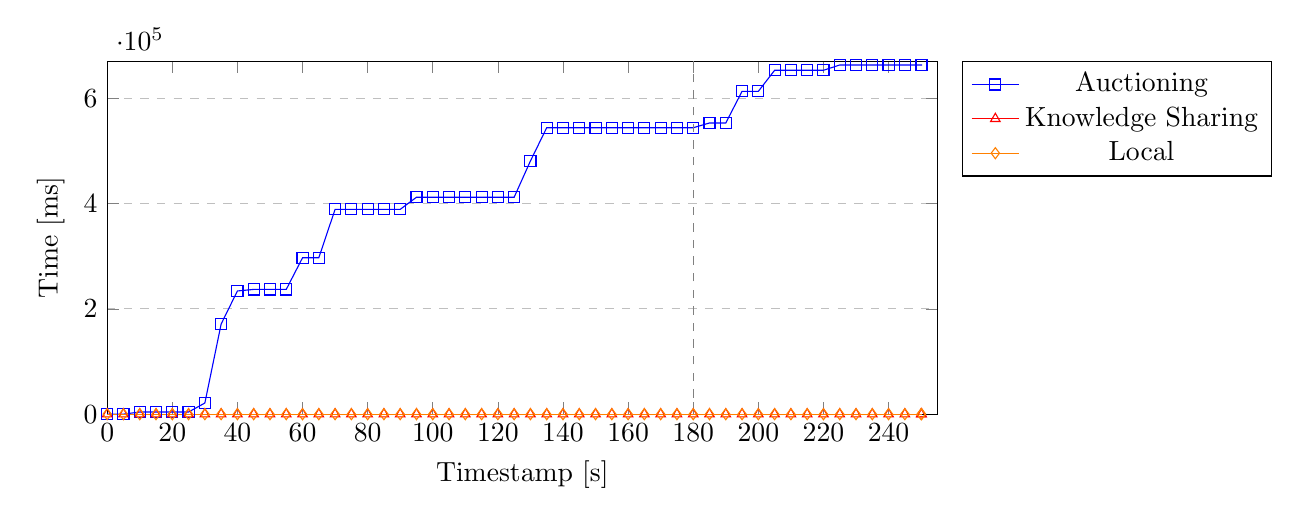
\begin{tikzpicture}
\begin{axis}[
    xlabel={Timestamp [s]},
    ylabel={Time [ms]},
    xmin=0, xmax=255000,
    ymin=0, ymax=670067,
    legend pos=outer north east,
    ymajorgrids=true,
    grid style=dashed,
    width=\textwidth,
    height=0.5\textwidth,
    scaled x ticks=base 10:-3,
    xtick scale label code/.code={}
]

	\addplot[color=blue,mark=square] coordinates {
        (0,0)(5000,64)(10000,4143)(15000,4143)(20000,4143)(25000,4143)(30000,21179)(35000,171183)(40000,233978)(45000,236929)(50000,236929)(55000,236929)(60000,297046)(65000,297049)(70000,388980)(75000,388980)(80000,388980)(85000,388980)(90000,388980)(95000,411980)(100000,411980)(105000,411980)(110000,411980)(115000,411980)(120000,411980)(125000,411980)(130000,480905)(135000,543951)(140000,543951)(145000,543951)(150000,543951)(155000,543958)(160000,543958)(165000,543962)(170000,543962)(175000,543962)(180000,543962)(185000,553054)(190000,553054)(195000,613073)(200000,613073)(205000,653079)(210000,653079)(215000,653087)(220000,653087)(225000,663101)(230000,663101)(235000,663101)(240000,663101)(245000,663101)(250000,663101)(250288,663101)
    };
    \addlegendentry{Auctioning}
	\addplot[color=red,mark=triangle] coordinates {
        (0,0)(5000,0)(10000,0)(15000,0)(20000,0)(25000,0)(30000,0)(35000,0)(40000,0)(45000,0)(50000,0)(55000,0)(60000,0)(65000,0)(70000,0)(75000,0)(80000,0)(85000,0)(90000,0)(95000,0)(100000,0)(105000,0)(110000,0)(115000,0)(120000,0)(125000,0)(130000,0)(135000,0)(140000,0)(145000,0)(150000,0)(155000,0)(160000,0)(165000,0)(170000,0)(175000,0)(180000,0)(185000,0)(190000,0)(195000,0)(200000,0)(205000,0)(210000,0)(215000,0)(220000,0)(225000,0)(230000,0)(235000,0)(240000,0)(245000,0)(250000,0)(250159,0)
    };
    \addlegendentry{Knowledge Sharing}
	\addplot[color=orange,mark=diamond] coordinates {
        (0,0)(5000,0)(10000,0)(15000,0)(20000,0)(25000,0)(30000,0)(35000,0)(40000,0)(45000,0)(50000,0)(55000,0)(60000,0)(65000,0)(70000,0)(75000,0)(80000,0)(85000,0)(90000,0)(95000,0)(100000,0)(105000,0)(110000,0)(115000,0)(120000,0)(125000,0)(130000,0)(135000,0)(140000,0)(145000,0)(150000,0)(155000,0)(160000,0)(165000,0)(170000,0)(175000,0)(180000,0)(185000,0)(190000,0)(195000,0)(200000,0)(205000,0)(210000,0)(215000,0)(220000,0)(225000,0)(230000,0)(235000,0)(240000,0)(245000,0)(250000,0)(250135,0)
    };
    \addlegendentry{Local}

	\addplot[color=gray, dashed,] coordinates {(180000,0) (180000,670067)};


\end{axis}
\end{tikzpicture}
    \caption{Graph showing the sum of time spent auctioning by agents in the risk introduction scenario.}
    \label{fig:auctioning-time-risk-introduction}
\end{figure}
\begin{figure}[H]
    \centering
        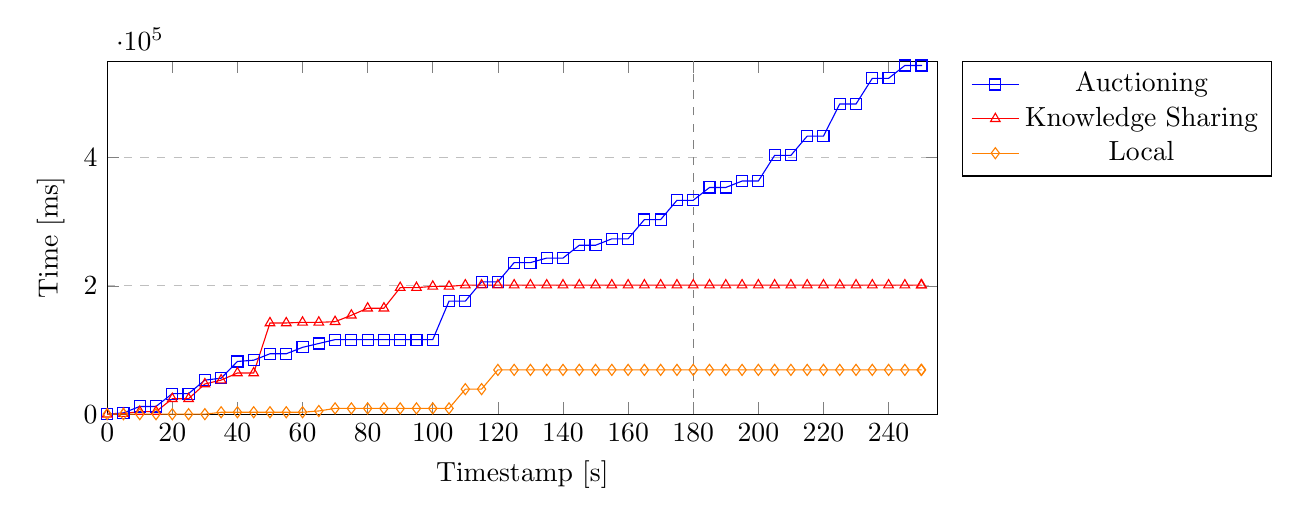
\begin{tikzpicture}
\begin{axis}[
    xlabel={Timestamp [s]},
    ylabel={Time [ms]},
    xmin=0, xmax=255000,
    ymin=0, ymax=550055,
    legend pos=outer north east,
    ymajorgrids=true,
    grid style=dashed,
    width=\textwidth,
    height=0.5\textwidth,
    scaled x ticks=base 10:-3,
    xtick scale label code/.code={}
]

	\addplot[color=blue,mark=square] coordinates {
        (0,0)(5000,2012)(10000,12058)(15000,12058)(20000,32063)(25000,32063)(30000,53081)(35000,56105)(40000,82157)(45000,84176)(50000,94183)(55000,94183)(60000,104190)(65000,110193)(70000,116237)(75000,116237)(80000,116237)(85000,116237)(90000,116237)(95000,116237)(100000,116237)(105000,176271)(110000,176271)(115000,206296)(120000,206296)(125000,236320)(130000,236320)(135000,243360)(140000,243360)(145000,263364)(150000,263364)(155000,273368)(160000,273368)(165000,303394)(170000,303394)(175000,333415)(180000,333415)(185000,353427)(190000,353427)(195000,363436)(200000,363436)(205000,403461)(210000,403461)(215000,433478)(220000,433478)(225000,483523)(230000,483523)(235000,523553)(240000,523553)(245000,543563)(250000,543563)(250288,543563)
    };
    \addlegendentry{Auctioning}
	\addplot[color=red,mark=triangle] coordinates {
        (0,0)(5000,1005)(10000,4021)(15000,4021)(20000,24028)(25000,24028)(30000,47052)(35000,53154)(40000,64163)(45000,64163)(50000,142192)(55000,142192)(60000,143196)(65000,143196)(70000,144197)(75000,154200)(80000,165206)(85000,165206)(90000,197224)(95000,197224)(100000,199232)(105000,199232)(110000,201240)(115000,201240)(120000,201240)(125000,201240)(130000,201240)(135000,201240)(140000,201240)(145000,201240)(150000,201240)(155000,201240)(160000,201240)(165000,201240)(170000,201240)(175000,201240)(180000,201240)(185000,201240)(190000,201240)(195000,201240)(200000,201240)(205000,201240)(210000,201240)(215000,201240)(220000,201240)(225000,201240)(230000,201240)(235000,201240)(240000,201240)(245000,201240)(250000,201240)(250159,201240)
    };
    \addlegendentry{Knowledge Sharing}
	\addplot[color=orange,mark=diamond] coordinates {
        (0,0)(5000,0)(10000,0)(15000,0)(20000,0)(25000,0)(30000,0)(35000,3017)(40000,3017)(45000,3017)(50000,3017)(55000,3017)(60000,3017)(65000,5025)(70000,9035)(75000,9035)(80000,9035)(85000,9035)(90000,9035)(95000,9035)(100000,9035)(105000,9035)(110000,39044)(115000,39044)(120000,69058)(125000,69058)(130000,69058)(135000,69058)(140000,69058)(145000,69058)(150000,69058)(155000,69058)(160000,69058)(165000,69058)(170000,69058)(175000,69058)(180000,69058)(185000,69058)(190000,69058)(195000,69058)(200000,69058)(205000,69058)(210000,69058)(215000,69058)(220000,69058)(225000,69058)(230000,69058)(235000,69058)(240000,69058)(245000,69058)(250000,69058)(250135,69058)
    };
    \addlegendentry{Local}

	\addplot[color=gray, dashed,] coordinates {(180000,0) (180000,550055)};


\end{axis}
\end{tikzpicture}
    \caption{Graph showing the sum of time spent adapting by agents in the risk introduction scenario.}
    \label{fig:adapting-time-risk-introduction}
\end{figure}

Figure \ref{fig:adapting-time-risk-introduction} shows that the knowledge-sharing agent is spending almost twice as much time adapting compared to the auctioning agent. Compared to figure \ref{fig:adapting-time-no-change} we see that the knowledge-sharing agent is spending more time adapting in the earlier stages of the scenario. More on this in subsection \ref{ssec:consecutive-runs}.
